\documentclass{article}

\usepackage{pdflscape}
\usepackage{hyperref}
\usepackage{graphicx}
\graphicspath{{images/}}

\title{Comparison of FPGA Development Kits}
\date{2015-07-09}
\author{J.D. McCormack}

\begin{document}
\begin{landscape}
\begin{center}

\begin{tabular}{||c c c c c c c c||}
	\hline
	Board Name  & Board Brand  & Chip Name & Chip Brand & MicroController  & Supplier & Price & link \\
	\hline\hline
	Mojo v3 & Embedded Micro  & Spartan 6 Lx9 & Xilinx & Yes (AT)&  Sparkfun & \$74.95 & 
	\href{https://www.sparkfun.com/products/11953}{Link}\\
	DEO-Nano & Altera & Cyclone IV & Altera & No &  Adarfuit & \$99.95 
	&\href{http://www.adafruit.com/products/451}{Link}\\
	Papilio Pro & Gadget Factory & Spartan 6 LX & Xilinx & Yes (AT) & Gadget Factory & \$84.99 & 
	\href{http://store.gadgetfactory.net/papilio-pro/}{Link}\\
	DE1 SOC Board & Altera & Cyclone V & Altera & Yes (ARM) & Altera & \$175.00 & 
	\href{http://wl.altera.com/education/univ/materials/boards/de1-soc/unv-de1-soc-board.html}{Link}\\
	DE2 115 & Altera & Cyclone IV & Altera &  No & Altera & \$309.00 & 
	\href{http://wl.altera.com/education/univ/materials/boards/de2-115/unv-de2-115-board.html}{Link}\\
	Zybo Zynq & Digilent & Zynq-7000 & Xilinx & Yes (ARM) & Digilent & \$125.00 & 
	\href{http://www.digilentinc.com/Products/Detail.cfm?NavPath=2,400,1198&Prod=ZYBO}{Link}\\
	Zedboard Zynq & Digilent & Zynq-7000 & Xlinx & Yes (Arm) & Digilent &  \$ 319.00 & 
	\href{http://www.digilentinc.com/Products/Detail.cfm?NavPath=2,400,1028&Prod=ZEDBOARD}{Link}\\
	Anvyl & Digilent & Spartan-6 & Xilinx & No & Digilent &  \$ 356.00 & 
	\href{http://www.digilentinc.com/Products/Detail.cfm?NavPath=2,400,1175&Prod=ANVYL}{Link}\\
	Nexys Video & Digilent & Atrix-7 & Xilinx & No & Digilent & \$299.00 &
	 \href{http://www.digilentinc.com/Products/Detail.cfm?NavPath=2,400,1475&Prod=NEXYS-VIDEO}{Link}\\
	Nexys 4-DDR & Digilent & Atrix-7 & Xilinx & No & Digilent & \$159.00 & 
	\href{http://www.digilentinc.com/Products/Detail.cfm?NavPath=2,400,1338&Prod=NEXYS4DDR}{Link}\\
	Basys 3 & Digilent & Atrix-7 & Xilinx & No & Digilent & \$79.00 & 
	\href{http://www.digilentinc.com/Products/Detail.cfm?NavPath=2,400,1288&Prod=BASYS3}{Link} \\
	\hline
\end{tabular}
\end{center}
\end{landscape}
	\newpage
	\section{Mojo V3}
	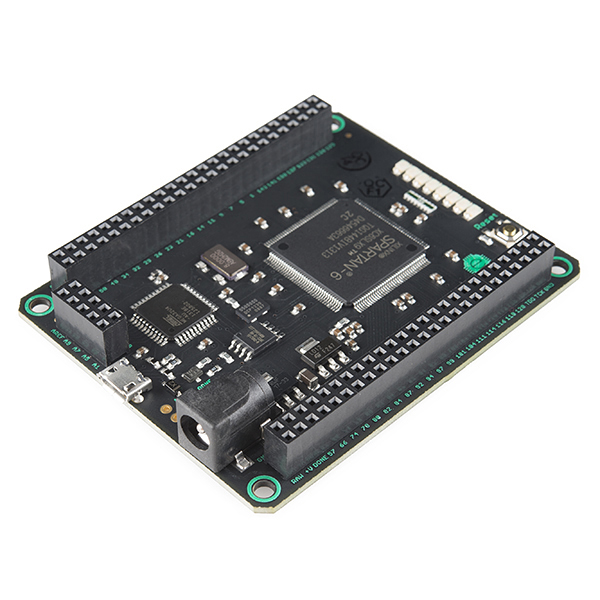
\includegraphics[scale=0.35]{mojo1}
	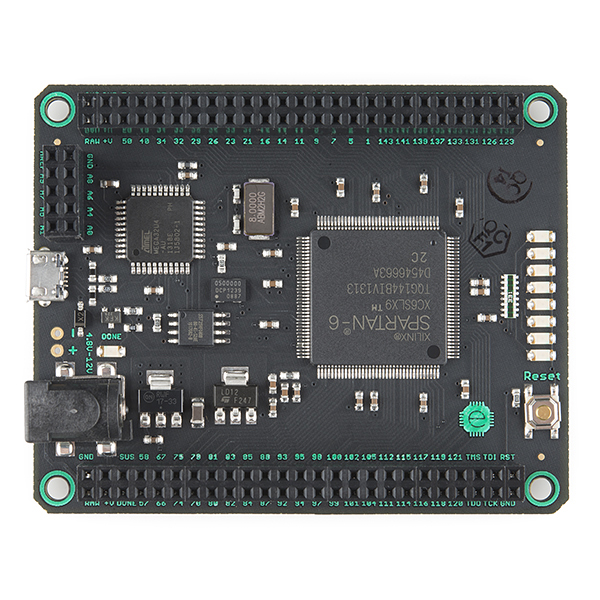
\includegraphics[scale=0.35]{mojo2}

	This FPGA is sold by sparkfun. Tutorials are provided by Embedded Micro, the developer. This is a small board featuring
	the Xilinx Spartan 6 and the Atmega32U. It features:
		\begin{itemize}
		\item 84 Digital IO Pins
		\item 8 Analog Inputs
		\item 8 GP LED's
		\item On Board voltage regulation
		\item on board flash memory
		\end{itemize}
	The tutorial documents can be found \href{https://embeddedmicro.com/tutorials/mojo/}{here}. The tutorials are written in
	Verilog. 
	
	\newpage
	\section{DE0-Nano}
	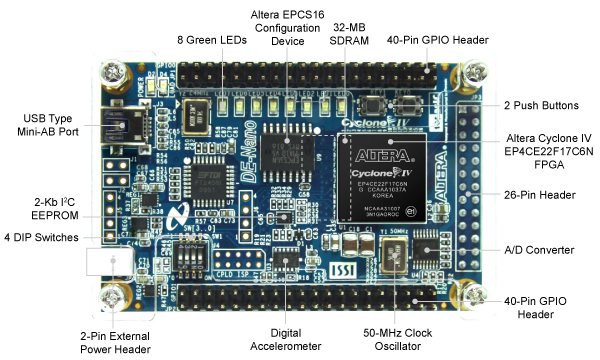
\includegraphics[scale=0.5]{de0}

	Another small form factor board. This board features an Altera Cyclone IV. It can be purchased through Altera or Adafruit
	Its feature list includes:
		\begin{itemize}
		\item 22,320 LEs
		\item 66 embeded 18 x 18 multipliers
		\item Built in USB-Blaster cable for programming the FPGA
		\item Three-axis accelerometer
		\item 8 channel, 12-bit A/D Converter
		\item 2 40 pin and 1 26 pin expansion header
		\item 32-MB SDram
		\item 2-Kb EEPROM
		\item 8 LEDs
		\item 4 Dip Switches
		\item 2 Push Buttons
		\item 50-MHz clock. 	
		\end{itemize}	
	The main training resources for Altera are online classes that require a fee to view. They can be found
	\href{https://www.altera.com/support/training/curricula.html}{here}.

	\newpage
	\section{Papilio Pro}
	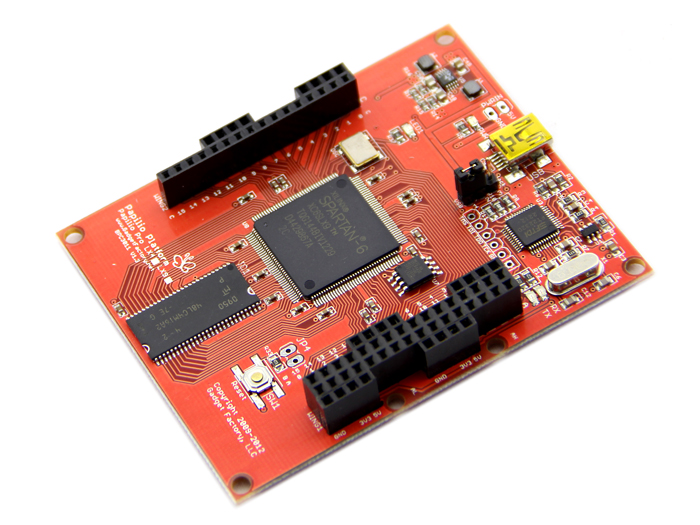
\includegraphics{ppro}
	I would not recommend this device as it seems to not have a lot of support. It is an oper source board
	however with schematics avaialable so it was included. It has an on board microcontroller which is nice.
	There are not many other features that would make this a better option over other designs. It uses a
	Xilinx Spartan 6 microcontroller. 

	\newpage
	\section{DE1-SoC Board}
	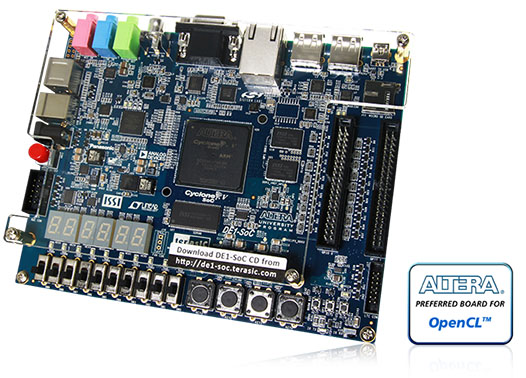
\includegraphics[scale=0.5]{de1}
	This is a great board from Altera. It has a lot of features. Since it is an SoC development board,
	it features both an FPGA and a Microcontroller. It features the Cyclone V FPGA and a dual core
	ARM Cortex-A9. Other features include:
		\begin{itemize}
		\item 85k LEs
		\item 4,450 kBits embedded memory
		\item 6 Fractional Phased Locked Loops (PLL)
		\item on board USB Blaster
		\item 64MB SDRAM on FPGA
		\item 1GB DDR3 SDRAM on microcontroller
		\item Micro SD Card socket
		\item USB to UART
		\item 10/100/1000 ethernet
		\item PS/2 mouse/keyboard
		\item IR Emitter/Reciever
		\item 2 40-pin expansion Headers
		\item 1 10-pin ADC Input Header
		\item VGA output and DAC
		\item 24-bit CODEC, line in, line out, microphon in
		\item NTSC/PAL/SECAM input TV Decoder
		\item 8 channel 12 bit ADC
		\item 4 user keys on FPGA
		\item 10 user switches on FPGA
		\item 10 LEDs on FPGA, 1 on MCU
		\item 2 microcontroller reset buttons
		\item six 7-segment displays
		\item G-sensor on microcontroller
		\end{itemize}
	Documentation and manuals are available 
	\href{http://www.terasic.com.tw/cgi-bin/page/archive.pl?Language=English&CategoryNo=165&No=836&PartNo=4}{here}
	
	\newpage
	\section{DE2}
	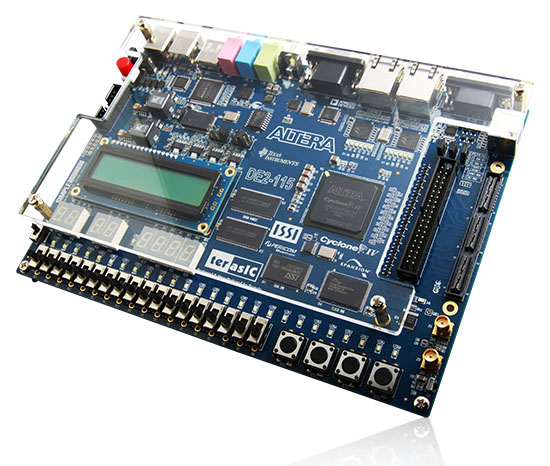
\includegraphics[scale=0.5]{de2}
	This is the next step up from the DE1 mentioned above. This is a nice board with a lot of on board peripherals.
	On this there is a Cyclone IV FPGA. However, this device does not have an on board microcontroller. The list of features
	includes:
		\begin{itemize}
		\item nearly 115k LEs
		\item 3,888 Embedded Memory
		\item 266 embedded 18x18 multipliers
		\item 4 general purpose PLLs
		\item 528 User IO's
		\item on board USB Blaster
		\item 128 MB SDRam
		\item 2MB SRam
		\item 8MB Flash
		\item 32Kbit EEProm
		\item 18 switches
		\item 4 push buttons
		\item 8 7 segment displays
		\item 24 bit CODEC, line in line out, microphone in jacks
		\item 16 x 2 LCD Display
		\item Three 50MHz clocks + SMAs for external clocks
		\item SD Card Slow
		\item 2 10/100/1000 Ethernet
		\item USB Type A and B
		\item 40 pin expansion port
		\item VGA-out connector
		\item DB-9 Serial Connector
		\item PS/2 Connector
		\item Infrared Reciever
		\item TV Decoder(NTSC/PAL/SECAM)
		\end{itemize}

		All resources and manuals are availbe
		\href{http://www.terasic.com.tw/cgi-bin/page/archive.pl?Language=English&CategoryNo=165&No=502&PartNo=4}{here}
	
	\newpage
	\section{Zybo Zynq}
	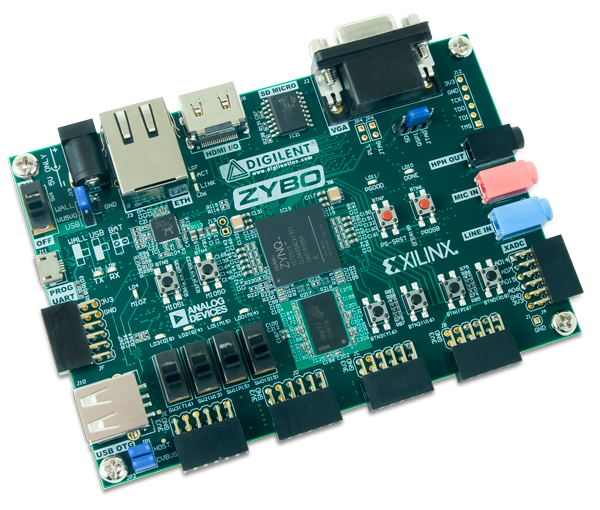
\includegraphics[scale=0.5]{ZYBO}
	This is a board based off of a Xilinx Zynq-7000 SoC. This board integrates a Xilinx 7-series FPGA with an ARM Cortex
	A9 microprocessor. This system also benefits from being a diglient board, meaning it is able to interface to
	Digilet's large number of expansion boards. Its features include:
	\begin{itemize}
	\item 650 MHz dual core A9 processor
	\item 512MB DDR3 Memory
	\item 10/100/1000 Ethernet
	\item USB 2.0
	\item SPI, UART, I2C
	\item Equivalent of an Artix-7 FPGA (28k logic cells)
	\item 12 bit, 2 channel ADC
	\item MicoSD slot
	\item 16 bit VGA output port
	\item Dual Role HDMI Port
	\item External EEPROM
	\item Audio Code with headphone, mic and line in
	\item On-board JTAG 
	\item on-board UART to USB 
	\item 6 push buttons
	\item 4 slide switches
	\item 5 LEDs
	\item 6 PMOD (proprietary add on board) connectors
	\end{itemize}
	
	There is a free PDF textbook to help people get started with this series of FPGA available
	\href{http://www.xilinx.com/support/university.html}{here}.

	\newpage
	\section{ZedBoard Zynq}
	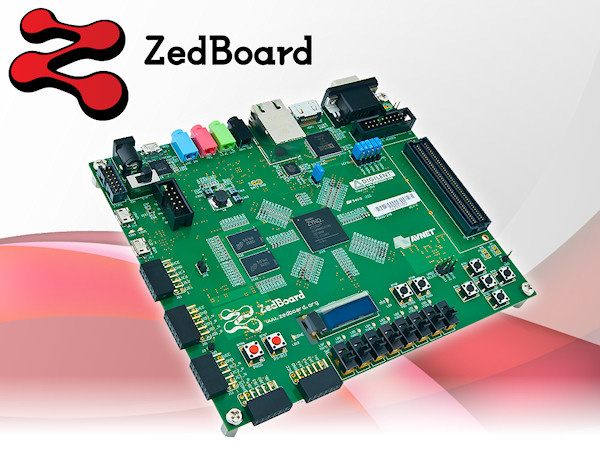
\includegraphics[scale=0.5]{ZedBoard}
	This is the big brother to the Zybo. Its a lot more expensive but provides more features. Again, it feautres
	the dual FPGA/Processor combo. 
	\begin{itemize}
	\item Zynq-7000 AP
	\item Dual Core ARM Cortex A9
	\item 512 MB DDR3
	\item 256 Mb Quad-SPI Flash
	\item 4 GB SD Card
	\item onboard USB-JTAG Programming
	\item 10/100/1000 Ethernet
	\item USB 2.0 and USB-UART
	\item PMOD controllers
	\item ADCs
	\item HDMI
	\item 8 bit VGA
	\item 128 X 32 OLED
	\item Audio Code
	\end{itemize}
	
	For some reason this device had less information on its listing than the previous one. It seems that it may 
	not be worth the extra cost versus the Zybo. This board is also part of the Xilinx University Program.
	 It would use the same online book as mentioned previously.

	\newpage
	\section{Anvyl}
	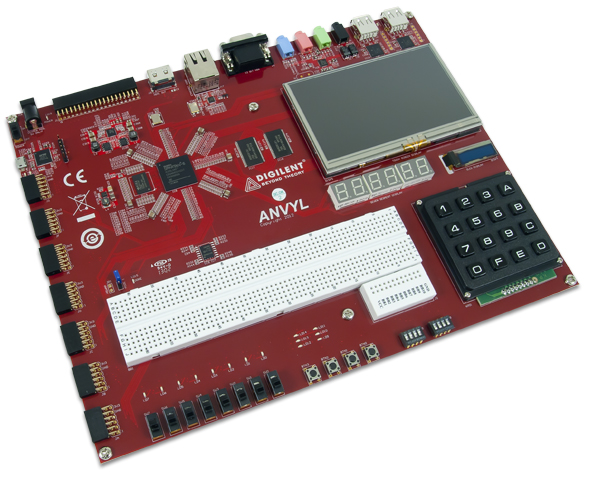
\includegraphics[scale=0.5]{ANVYL}
        
	This is a very large board with a lot of features. It is based off of the Sparan6 FPGA and does not feature
	an additional processor. The rest of its features include:

	\begin{itemize}
	\item Spartan6 FPGA with 45,000 LEs
	\item 128MB DDR SDRam 
	\item 2MB SRAM
	\item 16 MB FLASH
	\item 10/100 Ethernet
	\item HDMI Video Output
	\item 12 bit VGA Port
	\item 4.3" LED Backlit LCD
	\item 128x32 pixel 0.9" OLED Screen
	\item 3 two-digit 7 segment displays
	\item Audio Codec w/line in, out, mic, and headphone
	\item 100 MHz Crystal Oscillator
	\item USB2 ports for programming and HID (mouse/keyboard)
	\item USB-JTAG
	\item USB-UART
	\item Keypad with 16 labeled Keys (0-F)
	\item 14 LEDs
	\item 8 slide switches
	\item 8 DIP Switches
	\item 4 push buttons
	\item breadboard with 10 Digital I/O's
	\item 32 I/O's routed to 40 pin expansion connector
	\item 7 12-pin Pmod connecotrs
	\end{itemize}

	This board may not feature the fasted FPGA, or have an extra processor, but there is a LOT on the board.
	It would be very easy to make an entire semester's worth of projects with no external equipment at all.
	 This board is also supported by the Xilinx University Program. More information can be found 
	\href{http://www.xilinx.com/support/university/boards-portfolio/xup-boards/AtlysBoard.html}{here}.
	
	\newpage
	\section{Nexys 4 DDR}
	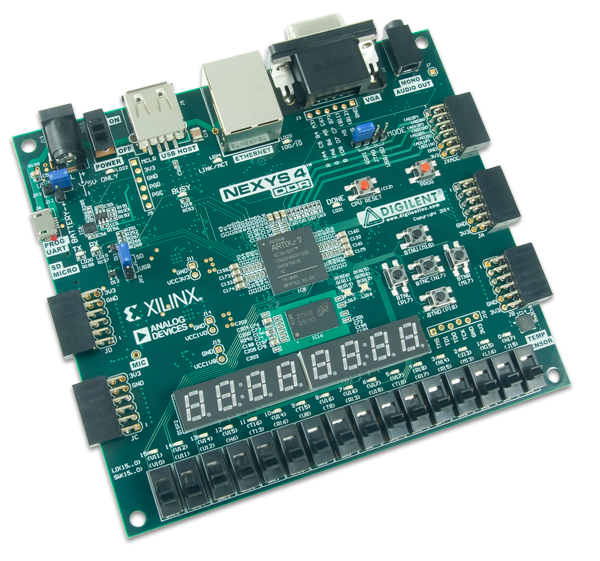
\includegraphics[scale=0.5]{Nexys4}

	This board is the successor to the board I used to learn FPGAs. These feature a decent selection of features
	for a reasonable price. There is a version just called the Nexys 4 that has been discontinued due to an EOL
	memory chip (hence the new name of DDR). The specifications for this board are:

	\begin{itemize}
	\item 100k LE's
	\item 4,860 kbits of RAM
	\item 240 DSP Slices
	\item on chip ADC
	\item 16 user switches
	\item USB-UART Bridge
	\item 12-bit VGA Output
	\item 3-axis accelerometer
	\item 128MiB DDR2
	\item Pmod for ADC signals
	\item 16 user LEDs
	\item Two PWM Tricolor LEDs
	\item PWM audio output
	\item Temperature Sensor
	\item Serial Flash
	\item USB-JTAG
	\item 2 4 digit 7 segment displays
	\item MicroSD card slot
	\item PDM Microphone
	\item 10/100 Ethernet
	\item Four Pmod Ports
	\item USB HID for mic, keyboard, memory sticks
	\end{itemize}
	
	As this is part of the Xilinx University Program, additional resources can be found 
	\href{http://www.xilinx.com/support/university/boards-portfolio/xup-boards/Nexys4BoardDDR.html}{here}.
	This is a good board with a lot of peripherals and a good amount of power. 	

	\newpage
	\section{Basys 3}
	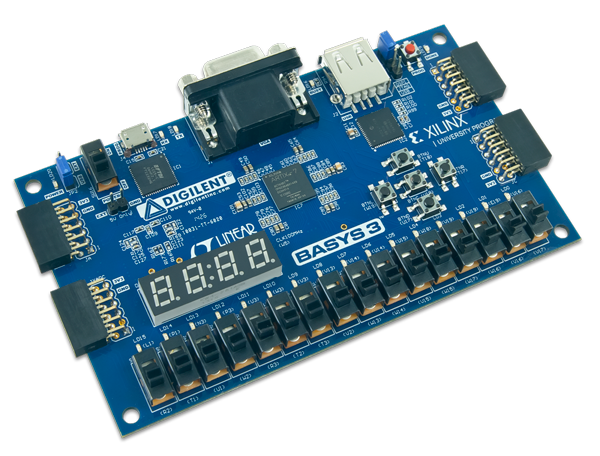
\includegraphics[scale=0.5]{Basys3}
	
	This is a cheaper board made by digilent. IT has less power and speed than the other boards but is only \$80.00. 
	This may be a good board for buying in large quantities, but will require more external peripherals than many of
	the other options. This is also part of the Xilinx University program, therefore additional resources can be
	found \href{https://www.digilentinc.com/Products/Detail.cfm?NavPath=2,400,1288&Prod=BASYS3}{here}. Its features
	include:

	\begin{itemize}
	\item 33k LE's
	\item 1,800 Kbits of RAM
	\item 5 clock management tiles with PLLs
	\item 90 DSP slices
	\item intenal clock speeds of 450 MHz
	\item on chip ADC
	\item 16 user switches
	\item 16 user LEDs
	\item 5 user pushbuttons
	\item 4-digit 7 segment displays
	\item 4 pmod connecotrs (1 with ADC connections)
	\item 12 bit VGA output
	\item USB-UART Bridge
	\item Serial Flash
	\item USB-JTAG
	\item USB HID Host for mice, keyboards, and memory sticks
	\end{itemize}
\end{document}
